\documentclass[a4paper]{article}
\usepackage{amssymb}
\usepackage{graphicx}

\title{H09M0A P\&D Embedded Systems and Multimedia}
\author{Seppe Iven - r0370830 \\ Koen Goetschalckx - r0375967}
\begin{document} 
\maketitle
\begin{center} Yu-Hui Huang, Johan Van Rompay, Hugo Van hamme
\end{center}

\section{Introduction}
This is an intermediate report about the matlab implementation of the P\&D assignment on subband coding, where a codec is implemented. The main techniques used to create such codec are subband filtering and adaptive quantisation, with the goal of compressing a stereo audio signal. This matlab implementation uses fixed point numbers and its parameters can be set in a flexible manner with the eye to optimal speech quality. \

TODO edit this paragraph to include all sections of the report:
This report contains a section on the main findings, an explanation about QMF filterbanks and the general matlab structure of the implementation of the assignment. It then explains the criteria for the optimal values of the parameters, followed by those values. Those values lead to a SNR and PESQ score for audio that has been encoded and decoded with this implementation.

\section{Main design specifications}
The following list contains the specifications that the design of the codec has to meet.

\begin{itemize}
\item It accepts stereo signals
\item The sampling frequency is 8 kHz
\item The bitrate is 24 kbit/s per channel codec, with good to very good speech quality
\item The implementation consists of a QMF tree-structured filterbank with polyphase implementation
\item An adaptive differential quantisation scheme should be used for every subband signal
\item The filterbank of the codec consists of a minimum of 4 subbands
\item The total delay of the coder and decoder must not exceed a certain threshold: the entire one way communication delay (ADC, coding, encryption, decryption, decoding, DAC) should be less than 150ms. This puts a maximum on the number of subbands, on the complexity of the filters and on the buffer size in the cryptography section. Note that the encryption and decryption functionality is provided by another group and is not a part of this assignment.

\end{itemize}

\section{Main findings}
Don' really know what to put here but the assignment said we need this section. Maybe this is an introduction/conclusion section?

\section{QMF and shizzle}
A Quadrature Mirror Filter, or QMF, is a special kind of filter that can be used to efficiently create a 2-way filter bank. Recursively applying QMFs as in figure \ref{fig:qmfrecursive} can split the signal into more subbands if wanted. QMF filters have some special properties:
\begin{itemize}
\item if $H_0(z)$ is a QMF filter, then $H_1(z) = H_0(-z)$ has the frequency response of $H_0$ mirrored around $\pi/2$.
\item if $H_0(z)$ is a QMF filter, then analysis filters $H_0(z)$ and $H_1(z) = H_0(-z)$ and synthesis filters $F_0(z)=H_1(-z)=H_0(z)$ and $F_1(z)=-H_0(-z) = -H_1(z)$ form an alias-free filter bank.
\end{itemize}
\begin{figure}[hbt]
\centering
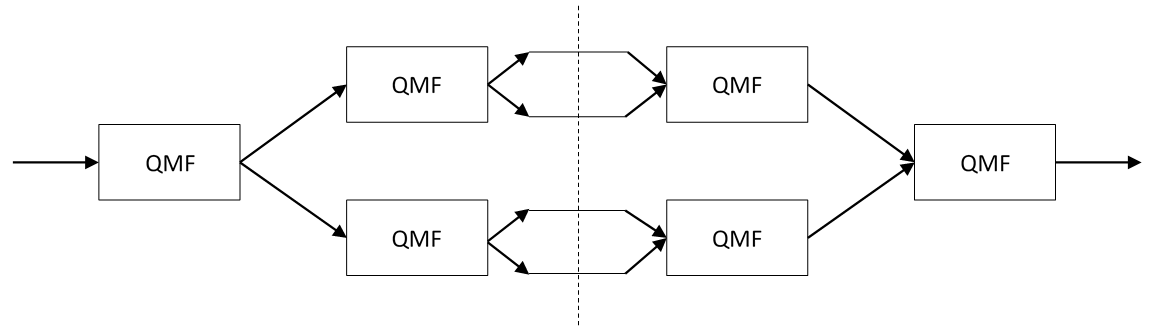
\includegraphics[width=.8\textwidth]{qmfrecursive}
\caption{4-way QMF filter bank by repeatedly applying QMF}
\label{fig:qmfrecursive}
\end{figure}
The second property indicates that $H_0(z)$ can completely define a alias-free QMF filter bank. For linear phase, this $H_0$ should be chosen symmetrical. Also, the filter should have an even amount of taps to avoid distortion at half the Nyquist frequency. The first property indicates that if $H_0$ is a good low-pass filter, then $H_1$ is a good high-pass filter.

Given these properties and constraints, a simple polyphase implementation for a QMF filter bank can be designed. Writing the polyphase decomposition of $H_0(z)$ as $E_0(z^2) + z^{-1} E_1(z^2)$ the decomposition of $H_1(z)$ is $E_0(z^2) - z^{-1} E_1(z^2)$. This lead to an efficient implementation, as shown in figure \ref{fig:qmf}.

For this project, both symmetric and asymmetric, where only one of the output bands of a QMF block are split further, structures were considered. Although 5 subbands, create by always splitting the lower frequency band, may possibly have lead to better results, further use and study of these asymmetric structured were cancelled as the teacher assistant said it these were not considered in the previous case and would lead to more complex C implementation. Thus, the final structure consists of QMF filter bank symmetricaly splitting the signal into four subbands, as in figure \ref{fig:qmfrecursive}.
\begin{figure}[hbt]
\includegraphics[width = \textwidth]{qmf}
\caption{Polyphase implementation of QMF filter bank}
\label{fig:qmf}
\end{figure}

TODO: show figure

TODO: bron vermelden? http://www.hindawi.com/journals/isrn/2013/815619/
Type something about how QMF works (so it can be skipped in get\_subbands.m). Talk about how many bits per subband, how this equals 24k bit/s etc..
TODO figures e.g. input and output signals of QMF system
TODO zeggen dat onderste subbanden belangrijker blijken uit testen -> meer bits aan toekennen
TODO over hoe we eerst 5 subbanden hadden (want onderste zijn belangrijker dan de rest), maar we er eigenlijk 4 moesten doen volgens die assistent

\section{Adaptive differential quantisation and shizzle}
TODO foto'ke van adaptive differential maar beter dan die in onze tekst.
TODO dit is lossy normaal dus vermelden
TODO delays implementeren want die afbeeding in het boek is ni goed 

\section{Matlab structure - Implementation overview}
This paper will now give a brief explanation of the matlab files that are used and their functionality.

TODO: Talk about all the scalings to make the numbers fit integers as much as possible etc

\subsection{generate\_some\_params.m}
This script can be run to generate the parameters that are used to call run.m

\subsection{run.m}
This is the main script that is used to divide an audio file into subbands, encode and decode those subbands, and synthesize them again to create an audio signal that closely resembles the original signal. Accepted audio files are .wav-files that are stereo or pairwise mono. The audio file that is used is that one named 'input.wav' TODO: Do we keep it this way or do we change input.wav to a parameter? 
\\
The input is scaled to a 16 bit integer. The input is then split into subbands by calling analysis.m. These subbands are first encoded by calling encoded.m and then decoded by calling decode.m. Finally, the subbands are combined by calling synthesis.m and the PESQ score for the reconstructed audio file is calculated.

\subsection{analysis.m}
This matlab script mainly splits the stereo (or pairwise mono) channels into separate channels, and feeds splits them into subbands by calling get\_subbands.m.

\subsection{get\_subbands.m}
This script recursively splits an audio channel into its subbands. It does this by applying polyphase QMF filters, as has been explained earlier in this paper TODO Is this true?. These filters are generated with a script that is given with the assignment and defined by its parameters.
TODO: Does this script also check for clipping/overflow?
\subsection{encode.m}
This script uses an adaptive differential quantisation method to compress an input signal. Such method is covered in an earlier part of this paper. TODO: Is this true?
TODO: Does this script also check for clipping/overflow?

This file also checks for clipping of values greater than 16 bits.

\subsection{decode.m}
This script is the inverse of encode.m: it takes the output of the adaptive differential quantisation function and constructs the original input signal.

\subsection{synthesis.m}
This script is the inverse of get\_subbands.m: its input are the separate subbands and it combines (synthesizes) them using the same QMF filters. Todo: These filters are the same, right?

\section{Criterion for optimal values}
From p127, we got the values for phi TODO we assumed gaussian distribution
Optimal values also includes: filter lengths etc just put here as many parameters as possible i guess

\section{Optimal values of all controllable parameters}
TODO hier onze finale waarden ingeven en zeggen hoe we eraan komen (zie boek: sommige vanuit theorie, sommigen bruteforce)
TODO also zeggen dat we optimised hebben voor de combined shizzle omdat die ons beter lijkt dan voor één aparte; dan zeggen wat de optimale en de minst optimale pesq waarden zijn bij de verschillende .wav bestandjes

\section{Final SNR \& PESQ}
TODO zeggen dat we SNR niet hebben gebruikt en daar een reden voor verzinnen bv pesq is beter

\section{Conclusion}
TODO spekken (zie taalgebruik van bossie) over alle secties die we behandeld hebben in deze paper
TODO zeggen dat we een goede maar niet finale matlab implementatie hebben (bv de deling die we nog aangepast hebben om op C te lijken; alsook dat onze final parameters nog niet final zijn maar subject to optimization)

\end{document}

TODO scan for codex instead of codec
TODO include total delay of code/encode: should be less than 150ms
TODO rechterdeel in run
TODO iets over delay?